\documentclass[12pt]{article}

\usepackage{fullpage}
\usepackage{epsfig}
\usepackage{graphicx}

\newcommand{\code}[1]{\texttt{#1}}

\author{Marc G. Bellemare, Adam White, Mike Sokolsky}
\title{The RLAI Robotic Simulator\\ A Tutorial}

\begin{document}
\maketitle

\section{Introduction}

This tutorial documents the RL-Glue version of the RLAI Robotic Simulator: how 
to install it, how to run it and how to use it in your work. Included is a 
Standalone mode, where you can personally control the robot in the environment.
After performing the installation (Section \ref{sec:installation}),  I suggest 
running the simulator in Standalone mode (Section \ref{subsec:standalone}) 
once initially to get an idea of the environment in which the robot lives.

This tutorial is divided into four parts in ordering of increasing depth of
use. The first part is concerned with the actual simulator package - how
to install and run the simulator. The second part explains how to use the 
simulator, in particular how to write an agent and an RL environment. It
also discusses how to use one of the other pre-defined environments. The
third part details how to create new simulator environments (e.g. the 
constituent parts of the simulator, as opposed to the RL-specific aspects)
and how to modify existing objects and create new ones. The last part focuses
on adding functionality to the simulator, for example how to design new 
sensors or how to improve the physics engine.

\subsection{Notes}

Running the simulator requires the following:

\begin{itemize}
\item{Java 1.5}
\item{A POSIX operating system such as Mac OS X, Linux or BSD (for running the additonal scripts)}
item{RL-Glue Core 3.0}
\end{itemize}

This tutorial does not discuss RL-Glue, on which this version of the simulator
is based. For more information about RL-Glue, you are encouraged to visit:

\begin{verbatim}
http://glue.rl-community.org
\end{verbatim}

On there you will find a link to download the most recent version of the RL-Glue
core, which is needed to run the simulator. The simulator itself is based
on the RL-Glue Java codec. For ease of use, we distribute the codec along
with this simulator. However, users are encouraged to install the RL-Glue
Java codec if they plan on developing for the simulator. 

\section{The Package}\label{sec:installation}

\subsection{Downloading the Package}

Each step of this section will be detailed with instructions for UNIX
systems. 

Along with this tutorial you should have downloaded a tarball of the 
RL-Glue version of the Simulator. If you have not yet done so, the Simulator
package can be found at

\begin{verbatim}
http://www.cs.ualberta.ca/~mg17/critterbot/files/RLGlueRLAISimulator.tgz
\end{verbatim}

For the remaining of this tutorial, I will assume that you have downloaded
this file to a directory called \verb+rlaisim+. Assuming that this 
is done, you should extract files from the tarball:

\begin{verbatim}
rlaisim> tar -xvzf RLAIRobotSimulator.tgz

<crunch crunch>

rlaisim> cd RLAIRobotSimulator
rlaisim/RLAIRobotSimulator>
\end{verbatim}

This will extract two directories, \code{RLGlueSim} and \code{example}.
The former contains the source for the abstract RL-Glue environment containing
the simulator; the latter contains example code that instantiates the
RL-Glue environment and provides a random agent and experiment.

\subsection{Building the RL-Glue Simulator Environment}

There are two parts to the RL-Glue Simulator Environment. The core part
encapsulates the RLAI Robotic Simulator into an abstract RL-Glue environment
which is then instantiated (the second part) into an environment with specific
action and observation spaces as well as a reward function.

In order to build the core environment and packaging it as a jar file, an
ant file has been provided:

\begin{verbatim}
rlaisim/RLAIRobotSimulator> cd RLGlueSim
rlaisim/RLAIRobotSimulator/RLGlueSim> ant build 

<crunch crunch>

BUILD SUCCESSFUL
Total time: 2 seconds
rlaisim/RLAIRobotSimulator/RLGlueSim>

\end{verbatim}

Provided everything went well, there should now be a file called RLGlueSim.jar
in the directory \code{RLGlueSim/products}. The next step is to copy it to
the example directory, so it can be used:

\begin{verbatim}
rlaisim/RLAIRobotSimulator/RLGlueSim> cp products/RLGlueSim.jar ../example/libs
\end{verbatim}

This completes the installation of the core RL-Glue simulator. The last
step is to return to the package root:

\begin{verbatim}
rlaisim/RLAIRobotSimulator/RLGlueSim> cd ..
rlaisim/RLAIRobotSimulator>
\end{verbatim}

\subsection{Running the Example}

With the package comes a full-fledged example containing an environment,
an agent (the random agent from the 
RL-Library\footnote{\code{http://rl-library.googlecode.com}}) and a 
sample experiment (also from the RL-Library). 

You should first ensure that the example code compiles. This can be done
by moving to the \code{example} directory and executing the script
\code{compile.sh}:

\begin{verbatim}
rlaisim/RLAIRobotSimulator> cd example
rlaisim/RLAIRobotSimulator/example> bash compile.sh

Compiled src/environment/DiscreteActionMapping.java src/environment/LightBasedRewardFunction.java src/environment/LightSensorsObservationMapping.java src/environment/SampleEnvironmentDescription.java src/environment/SampleSimulatorEnvironment.java src/environment/StandaloneSimulatorLoader.java
Compiled src/agent/RandomAgent.java
Compiled src/experiment/SampleExperiment.java

rlaisim/RLAIRobotSimulator/example>
\end{verbatim}

The script will warn you if compilation fails for some reason. Provided the
code does compile, you may either run the simulator in Standalone mode
(in which case you manually drive the robot) or run it via RL-Glue as a 
complete experiment.

\subsection{Running in Standalone Mode}\label{subsec:standalone}

The following will start the simulator in standalone mode:

\begin{verbatim}
rlaisim/RLAIRobotSimulator/example> bash runStandalone.sh 
\end{verbatim}

The \verb+runStandalone.sh+ script will compile the simulator loader,
\verb+src/environment/StandaloneSimulatorLoader.java+, and execute it. The 
specifics of this program will be detailed later in this tutorial.

Once you execute \verb+runStandalone.sh+, you should see a GUI appear, showing
the state of the simulator. The arrow keys will drive the robot around. Some 
of the
sensory information is currently drawn (such as bump sensors), but we do not
aim to provide a complete visualization of the data. You can also drive the
robot around using the ASDQWE keys, which provide three degrees of freedom
(by adding lateral motion). Figure \ref{fig:gui} shows a screenshot of
the simulator.

\begin{figure}\label{fig:gui}
\centerline{
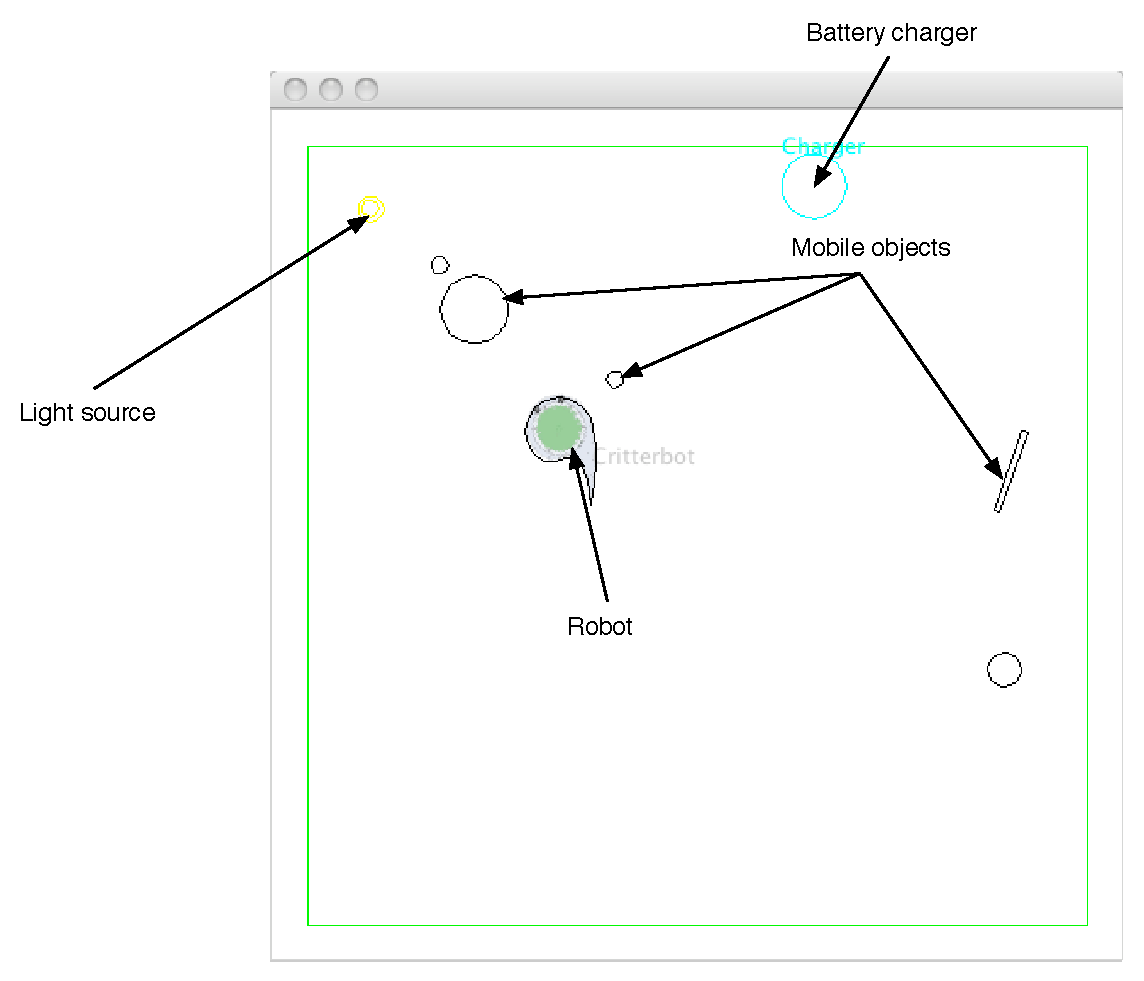
\psfig{file=images/Simulator_GUI.pdf,width=5in}
}
\caption{The RLAI Robotic Simulator Graphical User Interface.}
\end{figure}

You may find it inconvenient to recompile the source files every time. The
scripts provided in this package (including \code{runStandalone.sh}) take
command line arguments that modify the simulator behavior. In particular,
\code{-nc} will skip the compilation step and \code{-s} will specify a 
different time scale (with 1.0 being the default, and higher being faster)
at which the simulator should run. For example:

\begin{verbatim}
rlaisim/RLAIRobotSimulator/example> bash runStandalone.sh -nc -s 2.0
\end{verbatim}

will run the simulator without recompiling the source files in the
\code{example} directory and run at twice the real-time simulator speed.

\subsection{Running via RL-Glue}

The Standalone simulator does not actually require RL-Glue (in fact, you 
may have been able to proceed this far without even having RL-Glue installed).

Discuss how to run using RL-Glue

\end{document}
